\section{Model}\label{sec:model}
%Model - Drawing, equations, linear equations.
A free body diagram of the quadcopter is seen in \autoref{droneDiagram}. 
\begin{figure}[H]
	\centering
	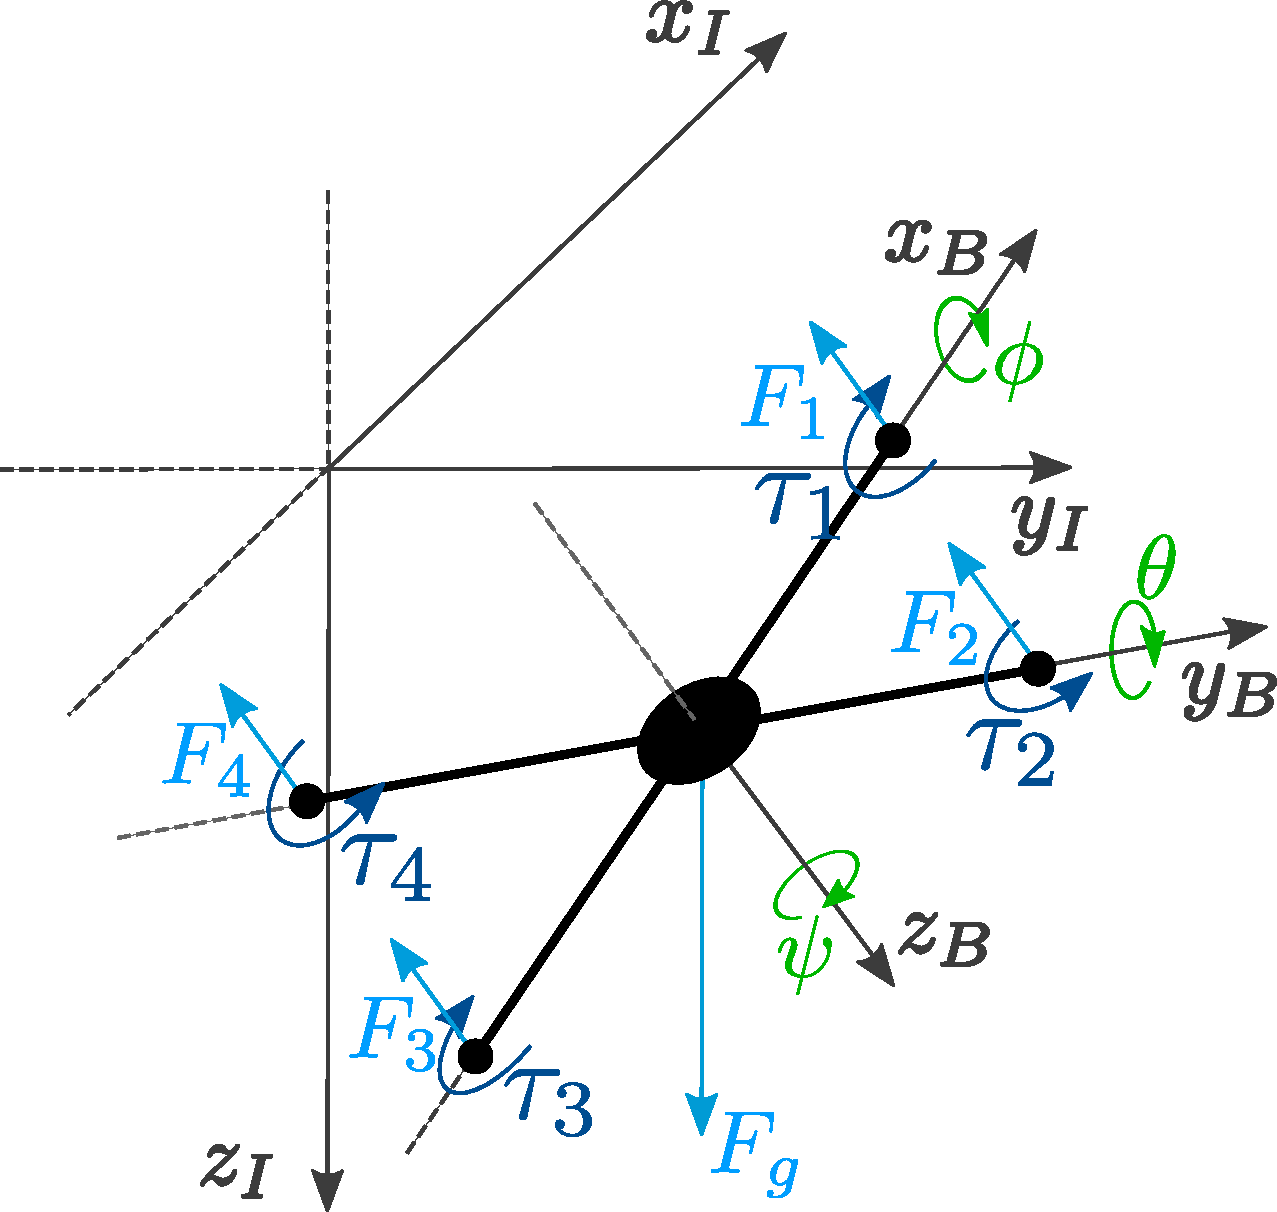
\includegraphics[width=.4\textwidth]{figures/droneDiagram}
	\caption{Forces ($\vec{F}_i$) and torques ($\vec{\tau}_i$) acting on the quadcopter and the positive references chosen for rotations and translations in both inertial and body coordinate frames.}
	\label{droneDiagram}
\end{figure}
%
As it is seen, the system is modeled by using two coordinate frames. The inertial frame is utilized to describe the translational movement while the body frame is attached to the quadcopter and used to characterize its attitude behavior. In the figure, also the positive references for rotational and translational movements are depicted, as well as the main forces and torques acting on the quadcopter. The positive rotations follow a right-hand fashion.

The forces generated in the propeller are readily obtained in the body coordinate frame. In order to represent them in the inertial frame a rotation matrix is used. It is built considering a 123 rotation sequence \cite{rotationmatrix}. This means that any rotation is described as three rotations around the $x_\mathrm{B}$ axis first, then around the $y_\mathrm{B}$ axis and lastly around the $z_\mathrm{B}$ axis. 
 
The dynamic model of the quadcopter is given by three sets of equations. The first describes the motor and the propeller, the second presents the attitude response of the quadcopter and the third explains how the translational variables of the system evolve.

\fxnote{In the modeling section, what are your assumptions? What is the reason for not including model parts such as Gyroscopic torque, Air friction/drag on the quadcopter itself (even though you include it on the propellers), Aerodynamic lift, Mass placement and separation of masses, Coriolis acceleration?}

\subsection{Motor and Propeller}
The four motors in the quadcopter generate a rotation in the propellers that creates the force that lifts the quadcopter. The thrust force can be modeled as proportional to the square of the motor rotational speed. The thrust coefficient for each motor is found experimentally.
 \fxnote{source on why the thrust and drag torque can be modelled like that.}
 
The rotation also generates a torque on each motor due to the aerodynamic drag. Drag torque is compensated in the quadcopter by having two of the motors turning in one direction and the two others in the opposite direction. It is also described as proportional to the square of the rotational speed in terms of a drag coefficient, which is also obtained experimentally.

The expressions for the thrust force and drag torque caused by the rotation of each propeller are
%
\begin{flalign}
	F&=k_{\mathrm{th}}\omega^2\label{eq:thrustForce}\\
	\tau&=k_{\mathrm{d}}\omega^2\label{eq:dragTorque}
\end{flalign}
%
\noindent where $F$ is the thrust force, $k_{\mathrm{th}}$ [\si{N s^2  rad^{-2}}] is the thrust coefficient, $\omega$ is the angular speed of the motor, $\tau$ is the drag torque and $k_{\mathrm{d}}$ [\si{N m s^2  rad^{-2}}] is the drag coefficient.
%\begin{where}
%  \va{F}{is the thrust force}{N}
%  \va{k_{th}}{is the thrust coefficient}{N\  s^2 \  rad^{-2}}
%  \va{\omega}{is the angular velocity}{rad s^-1}
%  \va{\tau}{is the drag torque}{N m}
%  \va{k_d}{is the drag coefficient}{N \  m\  s^2 \  rad^{-2}}
%\end{where}

These equations are used in the attitude and translational models presented below.
%
\subsection{Attitude Model}
The attitude model equations, which are based on Newton's Second Law for rotational movement, are as follows 
%
\begin{flalign}
	J_x\ddot{\phi}&=k_{\mathrm{th}} (\omega^2_4-\omega^2_2)  L \label{eq:AngleEqVelocities1}\\
	J_y\ddot{\theta}&=k_{\mathrm{th}} (\omega^2_1-\omega^2_3)  L \label{eq:AngleEqVelocities2} \\
	J_z\ddot{\psi}&=k_{\mathrm{d}} (\omega^2_1-\omega^2_2+\omega^2_3-\omega^2_4)\label{eq:AngleEqVelocities3}
\end{flalign}

\noindent where $J_x$, $J_y$ and $J_z$ are the moments of inertia around the three axes of rotation, $\ddot{\phi}$, $\ddot{\theta}$ and $\ddot{\psi}$ are the angular accelerations in roll, pitch and yaw, respectively, $\omega_i$ is the rotational speed of each motor and $L$ is the distance between the center of the quadcopter and the position of the motors. The parameters of the model are found in \autoref{sec:results}.

The expressions above state how the thrust forces and the drag torques generated on the propellers affect the attitude behavior of the quadcopter.  
\subsection{Translational Model}
The equations describing the response of the system along the inertial x, y and z axes are derived from Newton's Second Law of Motion. The forces that act on the system are those from the propellers and the gravitational force. These expressions are
%
\begin{flalign}
     m\ddot{x}_{\mathrm{I}} = &-k_{\mathrm{th}} ({\omega_1}^2+{\omega_2}^2+{\omega_3}^2+{\omega_4}^2) \label{eq:AccelerationEqInertial1}\\
     & \ \times (\cos\phi \sin\theta \cos\psi + \sin\phi\sin\psi)   \nonumber\\
     m \ddot{y}_{\mathrm{I}} = &-k_{\mathrm{th}}({\omega_1}^2+{\omega_2}^2+{\omega_3}^2+{\omega_4}^2) \label{eq:AccelerationEqInertial2}\\
     & \ \times (\cos\phi \sin\theta \sin\psi - \sin\phi \cos\psi)  \nonumber\\
     m\ddot{z}_{\mathrm{I}} = &F_g-k_{\mathrm{th}}\ ({\omega_1}^2+{\omega_2}^2+{\omega_3}^2+{\omega_4}^2) \label{eq:AccelerationEqInertial3}\\
     & \ \times \cos\phi\cos\theta  \nonumber
\end{flalign}
\noindent where $m$ is the mass of the quadcopter, $\ddot{x}_{\mathrm{I}}$, $\ddot{y}_{\mathrm{I}}$ and $\ddot{z}_{\mathrm{I}}$ are the accelerations along the inertial reference frame directions, $\phi$, $\theta$ and $\psi$ are the roll, pitch and yaw angles respectively and $F_g$ is the gravitational force acting on the quadcopter. The parameters of the model are found in \autoref{sec:results}.

It is worth mentioning that, as the thrust forces always point in the negative ${z}_{\mathrm{B}}$ direction, the accelerations along ${x}_{\mathrm{I}}$ and ${y}_{\mathrm{I}}$ directions are zero when pitch and roll angles are zero. 
\subsection{Linearization}
The model equations are linearized using the first order Taylor approximation around an equilibrium point of the system. This point is the hovering position, which implies that the attitude and translational accelerations and velocities are zero. The angular position of the quadcopter is also set to zero in the three angles.

Choosing a zero acceleration linearization point along the ${z}_{\mathrm{I}}$ axis yields an equilibrium rotational speed so that the necessary thrust is generated to compensate for the gravitational force. The relation is expressed as
\begin{flalign}
    \overline{\omega}_i=\sqrt{\frac{mg}{4k_{\mathrm{th}}}} \ \ \ .
    \label{eq:equilibriumomegas}
\end{flalign}
The resulting equations for the attitude model after the linearization are 
\begin{flalign}
  J_x \Delta\ddot{\phi}  = &2 k_{\mathrm{th}} L {\overline{\omega}_4} \Delta \omega_4 - 2\ k_{\mathrm{th}} L {\overline{\omega}_2} \Delta \omega_2
  \label{eqAngleLin1} \\
  J_y\Delta\ddot{\theta} =&2 k_{\mathrm{th}} L \overline{\omega}_1 \Delta \omega_1 - 2 k_{\mathrm{th}} L \overline{\omega}_3 \Delta \omega_3
  \label{eqAngleLin2} \\
  J_z\Delta\ddot{\psi}= &2 k_{\mathrm{d}} {\overline{\omega}_1} \Delta \omega_1 - 2 k_{\mathrm{d}}{\overline{\omega}_2} \Delta \omega_2 \label{eqAngleLin3}
  \\ & +\ 2\ k_{\mathrm{d}} {\overline{\omega}_3} \Delta \omega_3 - 2\ k_{\mathrm{d}} {\overline{\omega}_4} \Delta \omega_4\nonumber  
\end{flalign}
\noindent where $\Delta\ddot{\phi}$, $\Delta\ddot{\theta}$ and $\Delta\ddot{\psi}$ are the changes in rotational acceleration from the linearization point, $\overline{\omega}_i$ is the rotational speed of each motor to achieve equilibrium along the $z_\mathrm{I}$ axis and $\Delta \omega_i$ is the change in rotational speed of each motor from the linearization point. 

Similarly, the equations of the translational model are linearized. The result is
\begin{flalign}
  m\Delta\ddot{x}_{\mathrm{I}} =&-k_{\mathrm{th}} ({\overline{\omega}_1}^2+{\overline{\omega}_2}^2+{\overline{\omega}_3}^2+{\overline{\omega}_4}^2) \Delta\theta \label{eq:TransLinearEquations1} \\
  m\Delta\ddot{y}_{\mathrm{I}} = &\ \  \  k_{\mathrm{th}} ({\overline{\omega}_1}^2+{\overline{\omega}_2}^2+{\overline{\omega}_3}^2+{\overline{\omega}_4}^2) \Delta\phi \label{eq:TransLinearEquations2}\\
  m\Delta\ddot{z}_{\mathrm{I}} = &-2 k_{\mathrm{th}}\overline{\omega}_1 \Delta\omega_1 -2 k_{\mathrm{th}} \overline{\omega}_2 \Delta\omega_2 \label{eq:TransLinearEquations3} \\
 &\ \   -2 k_{\mathrm{th}} \overline{\omega}_3 \Delta\omega_3-2 k_{\mathrm{th}} \overline{\omega}_4 \Delta\omega_4 \nonumber 
\end{flalign} 
\noindent where $\Delta\ddot{x_{\mathrm{I}}}$, $\Delta\ddot{y_{\mathrm{I}}}$ and $\Delta\ddot{z_{\mathrm{I}}}$ are the changes in linear acceleration from the linearization point in each direction of the inertial frame and $\Delta \phi$ and $\Delta \theta$ are the changes in roll and pitch from the linearization point, respectively.